% !TEX root = calculus.tex


\chapter{DIFFERENTIATION}
\label{differentiation}

\athr Now our aim is a practical realization of the programme outlined in the previous dialogue. This dialogue could be considered as a drill on the calculation of derivatives. We shall divide the talk into three parts.
\begin{enumerate}
\item Differentiation rules.

\item Differentiation of elementary functions	$y = x^{2},	\, y	= \sin x, \,\, \text{and} \,\, y = \log_{a} x$. 
\item Application of differentiation rules to different functions.
\end{enumerate}

Before the start I would like to remind you that the differentiation of a function $f (x)$ is defined as the operation of obtaining $f' (x)$ from $f (x)$. This operation is performed by using the operator of differentiation $\dfrac{d}{dx}$
\begin{equation*}%
\frac{d}{dx} f(x) = f'(x)
\end{equation*}


\section*{The Differentiation Rules}
\label{diff-rules}
% sec 1 of 10

\athr \textbf{Rule One.} We shall prove the following theorem:
\begin{mytheo}{Theorem}
The derivative of the sum of two functions equals the sum of their derivatives provided that they exist, i.e.
\begin{equation}%
\frac{d}{dx} \left[f(x) + g(x) \right] = \frac{d}{dx} f(x)  + \frac{d}{dx} g(x) 
\label{deriv-sum}
% eq 1 of 10
\end{equation}
\end{mytheo}

Denote $f (x) + g (x) =u (x)$. Then the theorem can be written as follows: $u' (x) = f' (x) + g' (x)$. Try to prove this theorem.

\rdr First I write
\begin{align*}%
f' (x) & =\lim\limits_{\Delta x \to 0} \frac{f (x + \Delta x) - f(x)}{ \Delta x} \\
g' (x) & = \lim\limits_{\Delta x \to 0} \frac{g (x + \Delta x) - g(x)}{ \Delta x} \\
u'(x) & = \lim\limits_{\Delta x \to 0} \frac{u (x + \Delta x) - u(x)}{ \Delta x} \\
& = \lim\limits_{\Delta x \to 0}  \frac{f (x + \Delta x) + g (x + \Delta x) - f(x) - g(x)}{ \Delta x} \\
\end{align*}

But I don't know what to do next. 

\athr We shall repeat your writing but drop the limit signs:
\begin{align*}%
\frac{\Delta u(x)}{ \Delta x} & =  \frac{f (x + \Delta x) + g (x + \Delta x) - f(x) - g(x)}{ \Delta x} \\
& =  \frac{f (x + \Delta x)  - f(x) }{ \Delta x} +  \frac{g (x + \Delta x) - g(x)}{ \Delta x} \\
& = \frac{\Delta f(x)}{ \Delta x}  + \frac{\Delta g(x)}{ \Delta x} 
\end{align*}
This gives
\begin{equation*}%
\frac{\Delta u(x)}{ \Delta x}  = \frac{\Delta f(x)}{ \Delta x}  + \frac{\Delta g(x)}{ \Delta x} 
\end{equation*}

\rdr I see. Next we use the well-known theorem on the limit of the sum of functions, and the proof is complete. 

\athr Quite correct. \textbf{Rule Two.} Let us prove the
next theorem:
\begin{mytheo}{Theorem}
 A constant multiplier is factored out of the derivative, that is
\begin{equation}%
\frac{d}{dx} \left[a \, f(x) \right] =a \, \frac{d}{dx} f(x)
\label{deriv-const}
% eq 2 of 10
\end{equation}
\end{mytheo}
The theorem is immediately proved if we use the following obvious equality
\begin{equation*}%
\frac{\Delta \left[a \, f(x) \right]}{ \Delta x}  = a \, \frac{\Delta f(x)}{ \Delta x} 
\end{equation*}

\textbf{Rule Three.} Now we shall consider the theorem on the derivative of the product of two functions.
\begin{mytheo}{Theorem}
The derivative of a function $u (x) = f (x) \, \, g (x)$ is calculated
by using the following formula:
\begin{equation}%
 u' (x) = f' (x) \, g (x) + f (x) \, g' (x)
 \label{deriv-prod}
% eq 3 of 10
\end{equation}
provided that the derivatives $f' (x)$ and $g' (x)$ exist. 
\end{mytheo}
Formula \eqref{deriv-prod} is called the \emph{Leibnitz formula}. Another expression for the same formula is:
\begin{equation*}%
\frac{d}{dx} (f \, g) = g \, \frac{d}{dx} f  +  f \, \frac{d}{dx} g 
\end{equation*}
\rdr Apparently, as in the proof of the first theorem, we must express $\dfrac{\Delta u (x)}{\Delta x}$ through $\dfrac{\Delta f (x)}{\Delta x}$ and $\dfrac{\Delta g (x)}{\Delta x}$. But how to do it? 

\athr The simplest way is
\begin{align*}%
u + \Delta u & = (f + \Delta f) (g +  \Delta g)  \\
& = fg + g \Delta f + f \Delta g + \Delta f \Delta g
\end{align*}
Hence,
\begin{equation*}%
\Delta u = g \Delta f + f \Delta g + \Delta f \Delta g
\end{equation*}
 consequently,
\begin{equation*}%
\frac{\Delta u (x)}{\Delta x} = g(x) \frac{\Delta f (x)}{
\Delta x} +  f(x) \frac{\Delta g (x)}{\Delta x} +   \frac{\Delta f (x)}{
\Delta x} \Delta g(x)
\end{equation*}
 
 Now we find the limit for $\Delta x \to 0$. Notice that neither $g (x)$ nor $f (x)$ depends on $\Delta x $, and $\Delta g (x)$ tends to zero. As a result,
 \begin{equation*}%
\lim\limits_{\Delta x \to 0 } \frac{\Delta u (x)}{\Delta x} = \lim\limits_{\Delta x \to 0 } g(x) \frac{\Delta f (x)}{\Delta x} + \lim\limits_{\Delta x \to 0 } f(x) \frac{\Delta g (x)}{\Delta x}
\end{equation*}
  The theorem is thus proved. 
 
 \textbf{Rule Four.} The next theorem is related to the derivative
of the ratio of two functions. 
\begin{mytheo}{Theorem}
The derivative of a function $u (x) = \dfrac{f(x}{g(x)}$ is: 
\begin{equation}%
u' (x) = \frac{f'(x) g(x) - f(x) g'(x)}{g^{2} (x)}
 \label{deriv-div}
% eq 4 of 10
\end{equation}
provided that the derivatives $f' (x)$ and $g' (x)$ exist, and that $g (x) \neq 0$.
\end{mytheo}
It can be written in a different form:
 \begin{equation*}%
 \ddx \left(\dfrac{f}{g} \right) =\dfrac{g \ddx f - f \ddx g}{g^{2}}
\end{equation*} 
Try to prove this theorem.
 
\rdr I shall proceed by analogy with the preceding proof. I can write
Hence,
 \begin{align*}%
\Delta u & = \dfrac{f + \Delta f}{g + \Delta g} - \dfrac{f}{g} \\
& = \dfrac{g \dfrac{\Delta f}{\Delta x} - f  \dfrac{\Delta g}{\Delta x} }{g^{2} + g \Delta g}
\end{align*} 
 This yields,
 \begin{equation*}%
\frac{\Delta u}{\Delta x} = \dfrac{g \dfrac{\Delta f}{\Delta x} - f  \dfrac{\Delta g}{\Delta x} }{g^{2} + g \Delta g}
\end{equation*} 


Passing then to the limit for $\Delta x \to 0$, I take into account that neither $g$ nor $f$ depend on $\Delta x$, and that $\Delta g$ also tends to zero. Using the known theorems on the limit of the product and the sum of functions, we obtain
\begin{align*}%
\lim\limits_{\Delta x \to 0} \frac{\Delta u}{\Delta x} & = \lim\limits_{\Delta x \to 0} \left(\dfrac{ 1 }{g^{2} + g \Delta g}  \right) \,\, \lim\limits_{\Delta x \to 0} \left( g \dfrac{\Delta f}{\Delta x}  - f \dfrac{\Delta g}{\Delta x}  \right) \\
& = \frac{1}{g^{2}} \left( g \lim\limits_{\Delta x \to 0} \frac{\Delta f}{\Delta x} - 
f \lim\limits_{\Delta x \to 0} \frac{\Delta g}{\Delta x} \right)
\end{align*}
This completes the proof. 

\athr Very good. Now we shall discuss the, problem
of the differentiation of a \emph{composite function} (for composite functions, see \hyperref[more-on-function]{Dialogue Five}. Let $w = h (x)$ be a composite function, and $h (x) = g [f (x)]$. This composite function is the composition of two functions $w =	g (y)$ and $y  = f (x)$.

I remind you that the derivative $f' (x)$ indicates how faster $y$ charges compared to $x$ and the derivative $g' (y)$ indicates how faster $w$ changes compared to $y$.  Consequently, the product $g' (y) f' (x)$ must indicate how faster $w$ changes compared to $x$, i.e. it equals the derivative $h' (x)$.

\textbf{Rule Five.} Thus we arrive at the differentiation rule for
composite functions.
\begin{mytheo}{Theorem}
The derivative of a composite function $h (x) = g [f (x)]$ is:
\begin{equation}%
h' (x) = g' (y) \, f' (x)
 \label{deriv-comp}
% eq 5 of 10
\end{equation}
\end{mytheo}

\rdr We have arrived at this rule using very simple arguments. I wonder whether they can be regarded as a proof of the rule.

\athr No, of course not. Therefore I am going to give the proof of the differentiation rule for composite functions.

Let the independent variable $x$ have an increment $\Delta x$ such that $x + \Delta x$ belongs to the domain of $f (x)$. Then the variable $y$ will have an increment $\Delta y = f (x + \Delta x) - f (x)$, while the variable $w$ will have an increment $\Delta w = g (y + \Delta y) - g (y)$. Since the derivative $g' (y)$ exists.
the increment $\Delta w$ can be expressed as follows
\begin{equation*}%
\Delta w = g'(y) \Delta y + \eta \Delta y
\end{equation*}
where $\eta \to 0$ for $\Delta y \to 0$ (see expression (6) from the previous dialogue). 

Dividing both sides of the equation by $\Delta x$,	 we obtain
\begin{equation*}%
\frac{\Delta w}{\Delta x} = g'(y) \frac{\Delta y}{\Delta x} + \eta \frac{\Delta y}{\Delta x}
\end{equation*}
Next we pass to the limit for $\Delta x \to 0$
\begin{equation*}%
\lim\limits_{\Delta x \to 0} \frac{\Delta w}{\Delta x} = g'(y) \lim\limits_{\Delta x \to 0} \frac{\Delta y}{\Delta x} + \lim\limits_{\Delta x \to 0} \left( \eta \frac{\Delta y}{\Delta x} \right)
\end{equation*}
Since $\lim\limits_{\Delta x \to 0} \frac{\Delta w}{\Delta x} = h' (x)$ and $\lim\limits_{\Delta x \to 0} \frac{\Delta y}{\Delta x} = f'(x)$, we have
\begin{equation*}%
h'(x) = g'(y) \,\, f'(x) + f'(x) \lim\limits_{\Delta  x \to 0} \eta 
\end{equation*}
And since $\Delta y \to 0$ for  $\Delta x \to 0$, 
\begin{equation*}%
\lim\limits_{\Delta  x \to 0} \eta = \lim\limits_{\Delta  y \to 0} \eta = 0
\end{equation*}

Hence we arrive at \eqref{deriv-comp}, namely, at the rule for the differentiation of composite functions.

\textbf{Rule Six.} Finally, I shall give (without proof) the rule for the differentiation of inverse functions.

\begin{mytheo}{Theorem}
If a derivative $y' (x)$ of an initial monotonic function $y (x)$ exists and is not equal to zero, the derivative of the inverse junction $x (y)$ is calculated by the formula:
\begin{equation}%
x' (y) = \frac{1}{ y' (x)}
 \label{deriv-comp}
% eq 6 of 10
\end{equation}
\end{mytheo}

\rdr It seems that this formula can be easily obtained if we make use of the geometrical interpretation of the derivative. Really, consider the graph of a monotonic function $y (x)$ (\fig{fig-41}); its derivative at point $x_{0}$ is $\tan \alpha$. The same curve can, obviously, be regarded as the graph of the inverse function $x (y)$, with $y$ considered as the independent variable instead of $x$, and $x$ considered as the dependent variable instead of $y$. But the derivative of the inverse function at point $y_{0}$ is $\tan \beta$ (see the figure). 
\begin{figure}[!ht]%[13]{r}{0.5\textwidth}
\centering
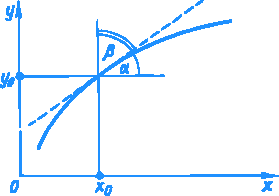
\includegraphics[width=0.6\textwidth]{figures/fig-41.pdf}
\caption{Derivative of a function and its inverse.}
\label{fig-41}
\end{figure}
Since $\alpha + \beta = \dfrac{\pi}{2}$ we have
\begin{equation*}%
\tan \beta = \frac{1}{\tan \alpha}
\end{equation*}

This gives the above-cited differentiation rule for inverse functions.

\athr I must admit that although your line of reasoning is not a rigorous mathematical proof, it is an example of an effective application of geometrical concepts.
\section*{The Differentiation of Functions \\
$y = x^{2}, \, y= \sin x, \, \, \text{and} \,\, y = \log_{a} x$}

\athr Using \eqref{note-1-def} from the previous dialogue, calculate the derivatives of the three indicated functions. Start with $y = x^{2}$. Go ahead.

\rdr I write
\begin{equation*}%
y + \Delta y = (x + \Delta x)^{2} = x^{2} + 2x	\Delta x + \Delta x^{2}
\end{equation*}
Hence, 
\begin{equation*}%
\Delta y =  2x	\Delta x + \Delta x^{2}
\end{equation*}
Consequently,
\begin{equation*}%
\frac{\Delta y}{\Delta x} =  2x	 + \Delta x
\end{equation*}
Further we pass to the limit for $\Delta x \to 0$
\begin{equation*}%
\lim\limits_{\Delta x \to 0} \frac{\Delta y (x)}{\Delta x} =  2x	
\end{equation*}
Therefore,
\begin{equation*}%
y' (x) = 2x
\end{equation*}

\athr You have thus obtained the result of applying the operator $\ddx$ to the function $y = x^{2}$:
\begin{equation}%
\boxed{
\ddx x^{2} = 2x}
\label{deriv-quad}
% eq 7 of 10
\end{equation}

We observe that for a quadratic function  $y = x^{2}$ at the input of the operator $\ddx$ we obtain a linear function $y = 2x$ at the output. 

Now try to differentiate the function $y = \sin x$. 

\rdr I shall write
\begin{equation*}%
y + \Delta y = \sin(x + \Delta x)^{2} = \sin x \cos \Delta x + \cos x \sin \Delta x 
\end{equation*}
Hence,
\begin{equation*}%
\Delta y = \sin x \cos \Delta x + \cos x \sin \Delta x - \sin x
\end{equation*}

\athr You had better use here the formula for the difference between two sines, not the formula for the sine of the sum. Represent $\Delta y$ in the form
\begin{equation*}%
\Delta y =  \sin(x + \Delta x) - \sin x = 2 \sin \frac{\Delta x}{2} \cos \left( x + \frac{\Delta x}{2} \right)
\end{equation*}
Next we obtain
\begin{equation*}%
\frac{\Delta x}{\Delta y} = \dfrac{ \sin \frac{\Delta x}{2}}{\frac{\Delta x}{2}} \cos \left( x + \frac{\Delta x}{2} \right)
\end{equation*}

In taking the limit for $\Delta x \to 0$, recall a result obtained in Dialogue Seven:
\begin{equation*}%
\lmts{\Delta x}{0} \frac{\sin \Delta x}{\Delta x} =1 
\end{equation*}

\rdr Yes, I see. Therefore,
\begin{align*}%
\lmts{\Delta x}{0} \frac{\Delta x}{\Delta y} & = \lmts{\Delta x}{0} \dfrac{ \sin \frac{\Delta x}{2}}{\frac{\Delta x}{2}} \lmts{\Delta x}{0} \cos \left( x + \frac{\Delta x}{2} \right) \\
& = \lmts{\Delta x}{0} \cos \left( x + \frac{\Delta x}{2} \right) \\
& = \cos x
\end{align*}

\athr The operator $\ddx$ applied to the function $y = \sin x$ thus generates the function $y = \cos x$:
\begin{equation}%
\boxed{ \ddx \sin x = \cos x}
\label{deriv-sin}
% eq 8 of 10
\end{equation}
Now we have to differentiate the function $y = \log_{a} x$. This time, however, we should start with a discussion of the transcendental number $e$ (which is usually called the ``base of natural or Napierian logarithms''). The number $e$ may be defined as the limit of a numerical sequence
\begin{equation}%
e  = \lmts{n}{\infty} \left( 1 + \frac{1}{n} \right)^{n}
\label{e-defn}
% eq 9 of 10
\end{equation}
The approximate value of e is: $e = \num{2.7182818284590}\ldots$
Using \eqref{e-defn}, we can show that $e$ is also the limit of $y = (1 + x)^{\dfrac{1}{x}}$ for $x$ tending to zero 
\begin{equation}%
\boxed{e  = \lmts{x}{0} \left( 1 + x \right)^{\dfrac{1}{x}}}
\label{e-defn2}
% eq 10 of 10
\end{equation}
We shall omit the proof of \eqref{e-defn2}. 

\rdr It seems that \eqref{e-defn2} follows logically from \eqref{e-defn}. 

\athr Far from it. Don't forget that in \eqref{e-defn} we deal
with the limit of a numerical sequence, while in \eqref{e-defn2} with the limit of a function at a point. While $n$ are integers, $x$ belongs to the real line (with the exception of $x = 0$). Therefore, the transition from \eqref{e-defn} to \eqref{e-defn2} requires a good deal of time and space.

Now turn to the differentiation of $y = \log_{a} x$. Follow the line adopted above. 

Start.

\rdr Obviously,
\begin{equation*}%
y + \Delta y = \\og_{a} (x+ \Delta x)
\end{equation*}
Hence,
\begin{align*}%
\Delta y & = \log_{a} (x+ \Delta x) -  \log_{a} x\\
& = \log_{a} \frac{x+ \Delta x}{ \Delta x}
\end{align*}
and, consequently,
\begin{equation*}%
\frac{\Delta x}{\Delta y} = \dfrac{ 1}{\Delta x} \log_{a} \frac{x + \Delta x}{x}
\end{equation*}
At this point I would have to find the limit for $\Delta x \to 0$. 

\athr I shall give you a hand here. We can rewrite
\begin{align*}%
\frac{\Delta x}{\Delta y} & = \log_{a} \left( \frac{x + \Delta x}{x} \right)^{\dfrac{1}{\Delta x}} \\
& =  \log_{a} \left( 1 + \frac{\Delta x}{x}  \right)^{\dfrac{x}{\Delta x} \cdot \dfrac{1}{x}} \\
& = \frac{1}{x} \log_{a} \left( 1 + \frac{\Delta x}{x} \right)^{\dfrac{ x}{\Delta x}}
\end{align*}

\rdr I see. This gives
\begin{equation*}%
\frac{\Delta x}{\Delta y}  = \frac{1}{x} \log_{a} \left( 1 + \frac{\Delta x}{x} \right)^{\dfrac{ x}{\Delta x}}
\end{equation*}
To find the limit for $\Delta x \to 0$, we use \eqref{e-defn2}. As a result 
\begin{align*}%
\lmts{\Delta x}{0} \frac{\Delta x}{\Delta y} & = \frac{1}{x} \lmts{\Delta x}{0}  \log_{a} \left( \frac{x + \Delta x}{x} \right)^{\dfrac{x}{\Delta x}} \\
& =  \frac{1}{x}  \log_{a} e \\
& =  \frac{1}{x} \cdot \frac{1}{\ln a}
\end{align*}
(symbol $\ln$ is the standard notation for the \emph{natural logarithm}).
 
\athr We have thus found that the operator $\ddx$ applied to the function $y = \log_{a} x$ gives $ y =  \dfrac{1}{x} \cdot \dfrac{1}{\ln a}$:
\begin{equation}%
\boxed{\ddx \log_{a} x  = \frac{1}{x} \cdot \frac{1}{\ln a}}
\label{deriv-log}
% eq 11 of 10
\end{equation}
Notice that the natural domain of the function $y =  \dfrac{1}{x} \cdot \dfrac{1}{\ln a}$ in \eqref{deriv-log} $] 0, \, \infty [$.

We can sum up our conclusions now. 
 
Using relation \eqref{note-1-def} from Dialogue Nine, first, we have established the six differentiation rules and, second, we have differentiated three functions. The results are summarized in \hyperref[diff-rules]{Table} on the next page, and \fig{fig-42} graphically represents the
result of the action of the operator $\ddx$ on the three selected
functions. The left-hand column in the figure lists the graphs of the three functions $f (x)$, and the right-hand column shows the graphs of the corresponding derivatives $f' (x)$.	


In what follows we shall not use formulas of type \eqref{note-1-def} from Dialogue Nine, that is, we shall not operate in terms of limit transitions. Using the results obtained above, we shall find the derivatives for a number of elementary functions without calculating the relevant limits.
\newpage 
\vspace*{1cm}

\begin{center}
\textcolor{DodgerBlue}{\textbf{The Differentiation Rules}}\\[30pt]
%{\smaller
\begin{tcolorbox}[colback=white,colframe=DodgerBlue]
%\boxed{
\begin{tabular}{p{5cm}>{\color{IndianRed}}l}
%\toprule
\textbf{Rule 1:} the differentiation of the sum of functions   & $\dfrac{d}{dx}(f + g) =  \dfrac{d}{dx}f + \dfrac{d}{dx} g $ \\
 \arrayrulecolor{DodgerBlue}\midrule
\textbf{Rule 2:} the differentiation of the function with constant term & $\ddx(af) = a \ddx f$ ($a$ = constant)\\
\midrule
\textbf{Rule 3:} the differentiation of the product of functions & $\ddx(fg) = f \ddx g + g \ddx f$\\
\midrule
\textbf{Rule 4:} the differentiation of the ratio of functions & $\ddx \dfrac{f}{g} = \dfrac{g \ddx f - f \ddx g }{g^{2}}$\\
\midrule
\textbf{Rule 5:} the differentiation of composite functions & $\ddx g[f(x)] = \left( \dfrac{d}{df} g(f) \right) \ddx f(x)$ \\
\midrule
\textbf{Rule 6:} the differentiation of inverse functions & $\dfrac{d}{dy} x(y) = \dfrac{1}{\ddx y(x)}$ 
%\bottomrule
\label{diff-rules}
\end{tabular}
%}
\end{tcolorbox}
\end{center}

\newpage


\begin{figure}[!ht]%[13]{r}{0.5\textwidth}
\centering
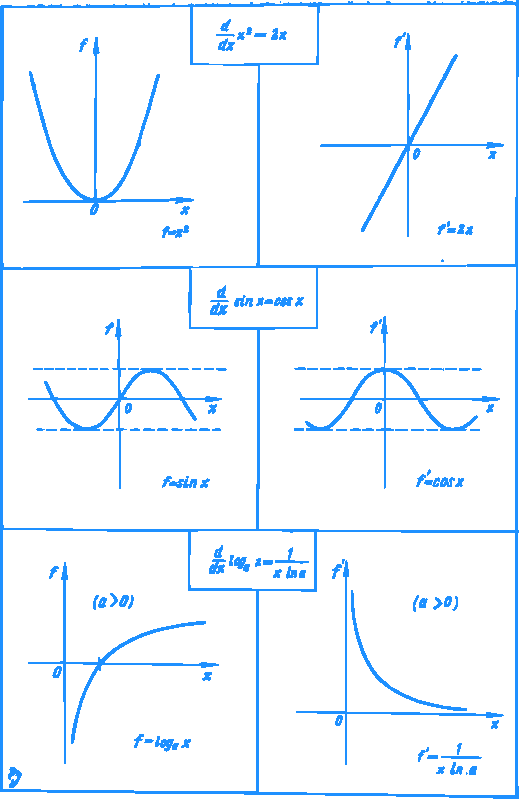
\includegraphics[width=.9\textwidth]{figures/fig-42.pdf}
\caption{Graphs of some basic functions and their derivatives.}
\label{fig-42}
\end{figure}


\section*{The Application of the Differentiation Rules to Different Functions}
\label{sec-3-9}

\athr As a first example, consider the function $y =x^{n}$. Prove that differentiation gives $y = n x^{n - 1}$ , that is,
\begin{equation}%
\boxed{\ddx x^{n}  = n x^{n-1}}
\label{deriv-power}
% eq 12 of 10
\end{equation}
Prove this proposition by using the \emph{method of mathematical induction}.

\rdr For $n = 2$ formula \eqref{deriv-power} holds and yields \eqref{deriv-quad}. Assume now that \eqref{deriv-power} holds for $n = m$. We have to prove that it is also true for $n = m +1$. We write $x^{m+1} = x^{m}\, x$ and use the \emph{Leibnitz formula} (\textbf{Rule Three}):
\begin{equation*}%
\ddx (x^{m}x) = x \ddx x^{m} + x^{m} \ddx x
\end{equation*}
Since $\ddx x = 1$ and according to the assumption $\ddx x^{m} = m x^{m-1}$, we obtain 
\begin{equation*}%
\ddx x^{m+1} = m x x^{m-1} + x^{m} = (m+1) x^{m}
\end{equation*}
The proof is completed. 

\athr The next example is the function $y = x^{-n}$.
Differentiate this function using \textbf{Rule Four} and \eqref{deriv-power}.


\rdr This is simple. Applying \textbf{Rule Four}, we obtain
\begin{equation*}%
\ddx \left( \frac{1}{x^{n}} \right) = \dfrac{-\ddx x^{n}}{x^{2n}}
\end{equation*}
By virtue of \eqref{deriv-power},
\begin{equation}%
\boxed{\ddx x^{-n}  = -n x^{-(n+1)}}
\label{deriv-power-neg}
% eq 13 of 10
\end{equation}
\athr One particular result that follows from \eqref{deriv-power-neg} is
\begin{equation}%
\boxed{\ddx \left( \frac{1}{x} \right)  = - \frac{1}{x^{2}}}
\label{deriv-power-neg}
% eq 14 of 10
\end{equation}
The next example is the function $y = \sqrt{x}$.

\rdr Here I shall use \textbf{Rule Six} (the differentiation rule for inverse functions). The inverse function involved is $x =y^{2}$. Its derivative is given by \eqref{deriv-quad}. As a result,
\begin{equation*}%
\ddx \sqrt{x} = \dfrac{1}{\ddx y^{2}} = \dfrac{1}{2y} = \dfrac{1}{2\sqrt{x}}
\end{equation*}
Thus
\begin{equation}%
\boxed{\ddx  \sqrt{x} = \dfrac{1}{2\sqrt{x}}}
\label{deriv-power-neg}
% eq 15 of 10
\end{equation}


\athr Now we can pass to the \emph{trigonometric} functions. Consider the function $y = \cos x$.

\rdr I propose to use \eqref{deriv-sin} and the identity $\sin^{2} x +  \cos^{2} = 1$. By differentiating both sides of the identity and using \textbf{Rule One}, we obtain
\begin{equation*}%
\ddx \sin^{2} x + \ddx \cos^{2} x = 0
\end{equation*}
Next, by applying \textbf{Rule Five} (the differentiation rule for composite functions) in conjunction with \eqref{deriv-quad}, we find
\begin{equation*}%
2 \sin x \ddx \sin x + 2 \cos x \ddx \cos x = 0
\end{equation*}
From \eqref{deriv-sin}, $\ddx \sin x= \cos x$ so that
\begin{equation*}%
\ddx \cos x = - \sin x 
\end{equation*}
\athr That is correct, although the result can be obtained in a simpler way. Better use the identity $\cos x = \sin \left(\dfrac{\pi}{2} -x \right)$. Further, applying \textbf{Rule Five}, we obtain
\begin{equation*}%
\ddx  \sin \left(\dfrac{\pi}{2} -x \right) = \left(\dfrac{d}{dy} \sin y \right) \ddx  \left(\dfrac{\pi}{2} -x \right)
\end{equation*}
(here  $y = \dfrac{\pi}{2} -x$)

Making use of \eqref{deriv-sin}, we find
\begin{equation*}%
\ddx  \sin \left(\dfrac{\pi}{2} -x \right) = - \dfrac{d}{dy} \sin y = - \cos y = - \sin x
\end{equation*}
Using now the suggested identity, we arrive at the final result:
\begin{equation}%
\boxed{\ddx  \sin x = - \cos x }
\label{deriv-sin}
% eq 16 of 10
\end{equation}

\rdr The operation of differentiation thus ``turns'' the sine into the cosine and, vice versa, that is, the cosine in to	 the sine.

\begin{figure}[!ht]%[13]{r}{0.5\textwidth}
\centering
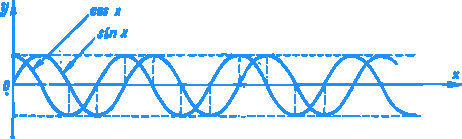
\includegraphics[width=\textwidth]{figures/fig-43.pdf}
\caption{Graphs of the sine and cosine functions.}
\label{fig-43}
\end{figure}

\athr. Yes, it does. But in the last case the sign changes too, that is, the cosine is transformed into the sine with a negative sign. If you plot the graphs of $\sin x$ and $\cos x$ in the same system of coordinates (\fig{fig-43}), you will find that at points $x$ where one of the functions reaches maximum or minimum (takes the value 1 or -1) the other function vanishes. It is readily apparent that this fact has
direct relation to your remark. If, for example, at a certain point $x$ the function $\sin x$ assumes its maximum value, the tangent to its graph at the same point will, obviously, be horizontal. 

Consequently, the derivative of the function (i.e, $\cos x$) must vanish at this point. I recommend that you carefully analyze \fig{fig-43}. In particular, follow the correspondence between the slope of the tangent to the graph of the function drawn at different points and the sign of the derivative at the same points.

Now turn to the next example, the function $y = \tan x$. Difierentiate this function using the results of the differentiation of $\sin x$ and $\cos x$ and applying \textbf{Rule Four}.

\rdr This will be easy:
\begin{align*}%
\ddx \left( \dfrac{\sin x}{\cos x} \right) & = \frac{\cos x \ddx \sin x - \sin x \ddx \cos x}{\cos^{2} x} \\
& = \frac{\cos^{2} x + \sin^{2} x}{\cos^{2} x} \\
& = \frac{1}{\cos^{2} x}
\end{align*}
Finally,
\begin{equation}%
\boxed{\ddx  \tan x = \frac{1}{ \cos^{2} x} }
\label{deriv-tan}
% eq 17 of 10
\end{equation}

\athr The result for $y = \cot x$ can be obtained similarly:
\begin{equation}%
\boxed{\ddx  \cot x = - \frac{1}{ \sin^{2} x} }
\label{deriv-tan}
% eq 18 of 10
\end{equation}
In order to differentiate $y = \arcsin x$, we use \textbf{Rule Six}
\begin{align*}%
\ddx \arcsin x & = \frac{1}{\dfrac{d}{dy} \sin y} \\
& = \frac{1}{\cos y} \\
& = \frac{1}{\cos \, (\arcsin x)}
\end{align*}
Since
\begin{equation*}%
\cos \, (\arcsin x) = \sqrt{1 - x^{2}}
\end{equation*}
 we obtain
\begin{equation}%
\boxed{\ddx  \arcsin x =  \frac{1}{ \sqrt{1 - x^{2} }}}
\label{deriv-arcsin}
% eq 19 of 10
\end{equation}
In order to differentiate $y = \arccos x$, it is sufficient to
use \eqref{deriv-tan} and the identity 
\begin{equation*}%
\arcsin x + \arccos x = \frac{\pi}{2}
\end{equation*}
Therefore,
\begin{equation}%
\boxed{\ddx  \arccos x = - \frac{1}{ \sqrt{1 - x^{2} }}}
\label{deriv-arccos}
% eq 20 of 10
\end{equation}
Using \textbf{Rule Six}, we differentiate the function $y = \arctan x$
\begin{align*}%
\ddx \arctan x & = \frac{1}{\dfrac{d}{dy} \tan y} \\
& = \cos^{2} y \\
& = [\cos \, (\arctan x)]^{2}
\end{align*}
Since 
\begin{equation*}%
\cos \, ( \arccos x ) = \frac{1}{ \sqrt{1 + x^{2}}}
\end{equation*}
we obtain
\begin{equation}%
\boxed{\ddx  \arctan x =  \frac{1}{ \sqrt{1 + x^{2} }}}
\label{deriv-arctan}
% eq 21 of 10
\end{equation}
And, finally, the differentiation of $y = \arccot x$ is carried out by using the identity
\begin{equation*}%
\arctan x + \arccot x = \frac{\pi}{2}
\end{equation*}
and yields
\begin{equation}%
\boxed{\ddx  \arccot x = - \frac{1}{ \sqrt{1 + x^{2} }}}
\label{deriv-arctan}
% eq 22 of 10
\end{equation}

We have thus performed the differentiation of all elementary trigonometric and inverse trigonometric functions,

 In conclusion, let us examine the exponential function $y = a^{x}$. Using \eqref{deriv-log} and \textbf{Rule Six}, we obtain
 
 This gives

\begin{equation}%
\boxed{\frac{d}{dx} a^{x} =  a^{x} \ln a}
\label{exp-deriv1}
% eq (23) of 10
\end{equation}

Result \eqref{exp-deriv1} is very interesting. We see that the differentiation of the exponential function $y = a^{x}$ again yields the exponential function $a^{x}$ multiplied by the constant term $\ln a$. In a particular case of $a= e$, we have $\ln e= 1$,and therefore
\begin{equation}%
\boxed{\frac{d}{dx} e^{x} = e^{x}}
\label{exp-deriv2}
% eq (24) of 10
\end{equation}
The exponential function $y = e^{x}$ is simply called the \emph{exponential curve}. From \eqref{exp-deriv2} it follows that differentiation transforms this function into itself.